\section{Method comparison against a no-pressure control}
\label{app:comparison}

In FourRooms, with the target \texttt{avoid\_bottom\_right}, the control and six of the seven methods end with higher mean forget-region occupancy than they started with, and the reward penalty at $\lambda=0.1$ ends where it started. Return rises over the same period and the shortest route to the goal passes through the region, so occupancy rises with competence whether or not anything is unlearned. The control that separates the two keeps the same scenario but uses its labels for evaluation only: continued PPO with no unlearning loss, no reward change and no masking. Figure~\ref{fig:control} and Table~\ref{tab:comparison} compare each method with it on seeds 42 to 46, paired by seed. Only the reward penalty at $\lambda=0.1$ excludes zero, and with seven comparisons it does not survive a Bonferroni correction. We report the comparison as an illustration of what the control changes, not as a ranking of methods.

\begin{figure}[h]\centering
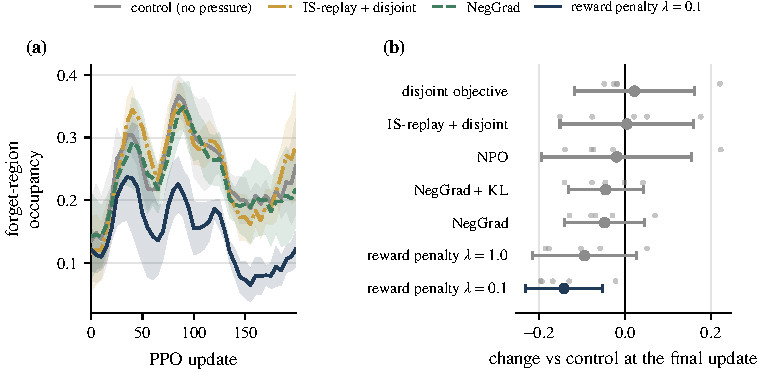
\includegraphics[width=\textwidth]{figures/fig_control.pdf}
\caption{\textbf{(a)} Forget-region occupancy during online unlearning, mean over five seeds with a $95\%$ CI band. The control rises with the others, because occupancy tracks task competence. \textbf{(b)} Change against the control at the final update, paired by seed, with $95\%$ intervals. Small dots are seeds.}
\label{fig:control}\end{figure}
\begin{table}[h]\centering\small
\caption{Final forget-region occupancy and return against the no-pressure control, paired by seed. $p$: paired $t$-test, uncorrected. $p_{\mathrm{Bonf}}$: multiplied by seven.}
\label{tab:comparison}
\begin{tabular}{@{}lccccc@{}}\toprule
Method & Seeds & $\Delta$ occupancy & $p$ & $p_{\mathrm{Bonf}}$ & $\Delta$ return \\ \midrule
disjoint objective & 5 & $+0.071$ & 0.319 & 1.00 & $-0.059$ \\
IS-replay + disjoint objective & 5 & $+0.066$ & 0.227 & 1.00 & $-0.090$ \\
NPO & 5 & $+0.035$ & 0.654 & 1.00 & $+0.046$ \\
NegGrad + KL anchor & 5 & $-0.007$ & 0.796 & 1.00 & $+0.015$ \\
NegGrad & 5 & $-0.020$ & 0.639 & 1.00 & $+0.016$ \\
reward penalty $\lambda=1.0$ & 5 & $-0.074$ & 0.221 & 1.00 & $-0.221$ \\
reward penalty $\lambda=0.1$ & 5 & $-0.113$ & 0.044 & 0.31 & $+0.012$ \\
\bottomrule\end{tabular}\end{table}

\section{Label scope: per-arm results}
\label{app:drift}

Table~\ref{tab:drift} gives the numbers behind Figure~\ref{fig:drift}. Agreement is measured on 4{,}000 states visited by each seed's baseline, with action sampling seeded so that the state set is identical across arms. Occupancy is the fraction of steps in the forget region over 16 evaluation episodes after the last update. $p$ values are paired $t$-tests over the fifteen seeds: for agreement, against the other-scope arm, and for occupancy, against zero.

\begin{table}[h]\centering\small
\caption{Each arm against the \texttt{matching\_steps} run on the same seed (mean, with standard deviation over seeds).}
\label{tab:drift}
\begin{tabular}{@{}llccccc@{}}\toprule
Domain & Arm & Labels changed & Agreement & $p$ & $\Delta$ occupancy & $p$ \\ \midrule
FourRooms & other scope & 20.0\% & 0.537 (0.062) & -- & $+0.046$ (0.074) & 0.030 \\
 & 1\% flips & 1\% & 0.601 (0.069) & 0.003 & $+0.019$ (0.064) & 0.263 \\
 & 10\% flips & 10\% & 0.591 (0.067) & 0.008 & $0.000$ (0.057) & 0.984 \\
 & baseline & -- & 0.544 (0.053) & -- & -- & -- \\
\midrule
CartPole & other scope & 32.6\% & 0.783 (0.147) & -- & $+0.023$ (0.351) & 0.805 \\
 & 1\% flips & 1\% & 0.746 (0.185) & 0.518 & $-0.066$ (0.244) & 0.310 \\
 & baseline & -- & 0.801 (0.141) & -- & -- & -- \\
\bottomrule\end{tabular}\end{table}

The label change is measured on one 2{,}048-step rollout of each seed's baseline, split into episodes as in training, and ranges over seeds from 11.2\% to 34.4\% in FourRooms and from 3.2\% to 72.5\% in CartPole. Compared directly with the 10\% control, the other scope's occupancy shift is larger by 0.046 ($p=0.06$).

